\chapter{结构学习}
\label{chap:pgm-structure-learning}

故障、过热和报警之间的连线若由领域知识给定，我们可以沿图估计参数、推断状态。现在只保留设备的运行记录，图本身也需要从数据中选择。所选连线能否表示变量依赖，箭头能否进一步解释为故障传播，是两个不同的问题：前者比较分布的表示，后者还要判断数据的产生机制及其他可能解释。

给定图时，局部概率关系决定联合分布的分解，参数学习再估计这些关系的数值（参见第~\ref{chap:pgm-directed}、\ref{chap:pgm-undirected}和\ref{chap:pgm-parameter-learning}章）。本章把未知量扩展到图结构。条件独立检验为连接提供局部证据，评分衡量候选模型的拟合与复杂度，搜索负责寻找合法候选。缺失观测和潜变量会改变可用证据；若要解释因果方向，还需加入相应机制假设。

\section{结构学习的定义}
\label{sec:pgm-structure-learning-definition}

我们从同一组变量的完整记录开始。记节点集合为$V=\{1,\ldots,d\}$，随机向量为$\bm{X}=(X_1,\ldots,X_d)^{\top}$，数据为$\mathcal{D}=\{\bm{x}_r:r=1,\ldots,n\}$，暂取样本独立同分布。给定候选图族$\mathfrak{G}$及各图对应的分布族$\mathcal{M}(\mathcal{G})$，\term{结构学习}（structure learning）利用数据和领域知识选择或评价依赖关系的图表示。候选范围可以规定边的类型，也可以限制父集大小、禁止特定边或仅允许树；缺失数据及多干预环境随后另行处理。

学习结果应表示数据能够确定的信息。用于预测时，可以选择拟合与复杂度折中的图；保留不确定性时，可以给出结构后验；高斯条件依赖可以用稀疏精度矩阵表示。若多张图在可用信息下无法区分，结果就应保留它们的共同关系。这些输出对应不同统计目标，并非把同一个确定结果换一种画法。

有向图的方向首先受到条件独立信息的限制。具有相同d-分离关系的有向无环图组成\term{Markov等价类}（Markov equivalence class, MEC）。两图等价恰好要求：忽略方向后的邻接关系，即\term{骨架}（skeleton），相同；$i\to k\leftarrow j$且$i,j$不相邻的\term{无屏蔽碰撞结构}（unshielded collider，又称v-structure），也相同。这里比较图所蕴含的全部独立关系，区别于特定参数抵消产生的额外独立性；完整刻画见图模型教材\scite{pgm-koller2009}

局部条件分布没有额外函数形式限制时，等价图表示相同的分布族。例如$X_1\to X_2\to X_3$、$X_1\leftarrow X_2\leftarrow X_3$和$X_1\leftarrow X_2\to X_3$都只要求$X_1\perp X_3\mid X_2$。将两条边同时指向$X_2$则得到碰撞图，它要求两端边缘独立，属于另一个等价类。图~\ref{fig:pgm-structure-learning-equivalence}对照这些方向，展示三种表示共同确定的关系。

一张图也可以直接保留整个等价类的信息。\term{完成的部分有向无环图}（completed partially directed acyclic graph, CPDAG）将类内共同的方向画成箭头，将其余边画成无向边，也称观测本质图。未定向边的合法选择相互约束：补全必须保持无环且不增加无屏蔽碰撞。因此，“恢复CPDAG”表示恢复类内不变的关系；任取代表图所增加的方向仍属选择，而非新增数据证据。

\begin{figure}[htbp]
  \centering
  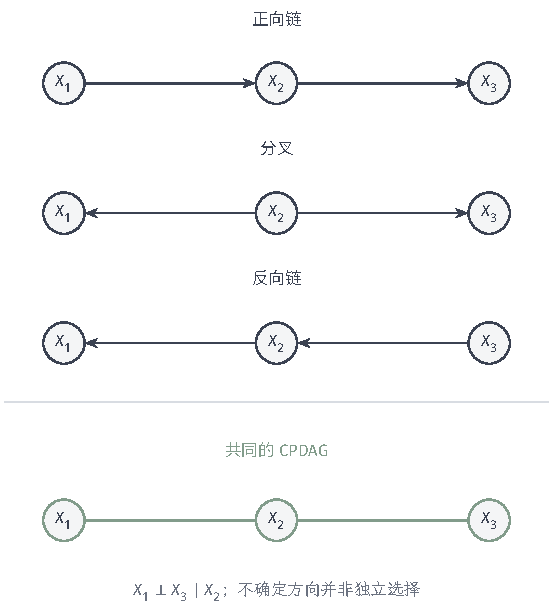
\includegraphics[width=93.652mm]{figures/06-probabilistic-graphical-models/03-learning/tikz/pgm-structure-learning-equivalence/figure.pdf}
  \caption{三种无碰撞有向图的等价表示。它们的骨架及条件独立关系相同，底部CPDAG保留这些共同信息；无向边表示类内方向可变。定向时两边须共同考虑：若都指向$X_2$，就会引入新碰撞，离开原等价类。}
  \label{fig:pgm-structure-learning-equivalence}
\end{figure}


候选空间还决定学习的计算规模。$d$个节点共有$2^{\binom d2}$种简单无向图；有向无环图即使固定拓扑序，也有这么多种边集。潜变量边缘化后的混合图允许不同端点标记，还受到整体合法性约束。扩大图族会增加可表示的分布，也增加参数、样本和搜索需求。频繁推断时，可把树宽等计算性质列为候选限制，并说明它们来自计算预算。

\section{有向图结构学习}
\label{sec:pgm-structure-learning-directed}

在有向图中，我们可以用条件独立检验考察局部联系，也可以用似然及复杂度为整张图评分。搜索算法随后根据这些证据寻找候选：它既可使用一种证据，也可组合两种证据。因此，检验和评分规定怎样比较结构，搜索规定怎样执行比较，三者可以配合使用。

\subsection{条件独立约束}
\label{sec:pgm-structure-learning-constraints}

由独立性删边，需要让独立关系确实反映图结构。\term{忠实性}（faithfulness）要求分布的条件独立与图上的d-分离一致，排除参数抵消带来的额外独立性。若集合$S\subseteq V\setminus\{i,j\}$使$X_i$与$X_j$条件独立，在该假设下便可删去$i,j$之间的边。总体分布未知时，算法实际检验的是
\[
  H_0:X_i\perp X_j\mid\bm{X}_S,
\]
并在未拒绝$H_0$时暂时删边。有限样本的检验功效会限制这一步：真实依赖过弱时也可能未被检出，因此未拒绝只是当前证据，尚未证明独立。

离散记录可以按条件配置分层计数。令$N_{a,b,s}$统计$(X_i,X_j,\bm{X}_S)=(a,b,s)$的次数，点号表示对相应指标求和。比较联合频率与独立假设下的频率，得到似然比统计量
\begin{equation}
  G^2=2\sum_{a,b,s:N_{a,b,s}>0}
  N_{a,b,s}\log
  \frac{N_{a,b,s}N_{\cdot,\cdot,s}}
       {N_{a,\cdot,s}N_{\cdot,b,s}}.
  \label{eq:pgm-structure-learning-g-test}
\end{equation}
各单元概率为正、状态数固定且样本足够时，原假设下的统计量渐近服从卡方分布。若条件变量有$q_S$种配置，自由度为$q_S(r_i-1)(r_j-1)$，$r_i,r_j$是两端状态数。结构性零单元、稀有配置及小样本都可能破坏近似，检验校准需与这些条件一起检查。

还可以直接衡量各条件配置中的分布差异。\term{条件互信息}（conditional mutual information）比较条件联合分布与条件边缘的乘积；有限离散情形为
\[
  I(X_i;X_j\mid\bm{X}_S)
  =\sum_{a,b,s}p(a,b,s)
       \log\frac{p(a,b\mid s)}{p(a\mid s)p(b\mid s)}.
\]
正概率项构成各条件配置下KL散度的加权平均，故此量非负，且为零恰好表示条件独立。代入经验频率可得$\widehat I=G^2/(2n)$。$S$为空时，它成为\term{互信息}（mutual information），衡量边缘依赖；这种依赖可能通过其他变量传递，未必对应直接边。

联合高斯分布提供了另一个计算入口。分别将两端对$\bm{X}_S$作线性回归，残差的相关系数就是偏相关$\rho_{i,j\mid S}$；在非退化高斯设定中，它为零等价于条件独立。对样本偏相关$\widehat\rho$作Fisher变换，得到
\[
  Z=\frac{\sqrt{n-|S|-3}}{2}
    \log\frac{1+\widehat\rho_{i,j\mid S}}
                  {1-\widehat\rho_{i,j\mid S}},
\]
在原假设$\rho_{i,j\mid S}=0$下，取$n>|S|+3$且相应渐近近似适用时，$Z$近似服从标准正态分布。非高斯数据中的零偏相关只排除某类线性关系，需要更丰富的统计信息才能检验条件独立。核检验可用于非线性关系，其结论仍依赖核、正则化及零分布校准；一般回归残差不相关也不足以替代原变量条件独立。

下面用同一张计数表比较检验、评分和搜索。取三个二值测量量$X_1,X_2,X_3$，可以把它们理解为设备的状态指示，数值则重新构造。表~\ref{tab:pgm-structure-learning-counts}含100条教学记录，各变量的$0$和$1$均出现50次，未使用真实测量数据或前章故障模型参数。

\begin{table}[htbp]
  \centering
  \begin{tabular}{ccc r@{\qquad}ccc r}
    \toprule
    $x_1$ & $x_2$ & $x_3$ & 次数 & $x_1$ & $x_2$ & $x_3$ & 次数 \\
    \midrule
    0 & 0 & 0 & 36 & 1 & 0 & 0 & 4 \\
    0 & 0 & 1 & 9  & 1 & 0 & 1 & 1 \\
    0 & 1 & 0 & 1  & 1 & 1 & 0 & 9 \\
    0 & 1 & 1 & 4  & 1 & 1 & 1 & 36 \\
    \bottomrule
  \end{tabular}
  \caption{100条人工二值记录。一种生成表示是：从公平根变量出发，沿两条边分别以$0.1$、$0.2$的概率独立翻转。该表示恰好产生表中频率；其他观测等价方向也可产生同一分布，因果方向因而尚未确定。}
  \label{tab:pgm-structure-learning-counts}
\end{table}

记经验频率为$\widehat p$。两端的联合频率$\widehat p(X_1=1,X_3=1)=0.37$，超过边缘乘积$0.25$，显示边缘依赖。固定$X_2=0$后，一格条件频率却可写成
\[
  \widehat p(X_1=0,X_3=0\mid X_2=0)
  =\frac{36}{50}=\frac{45}{50}\frac{40}{50}.
\]
其余三格以及$X_2=1$层也满足乘积分解，因此经验条件互信息和$G^2$均为零（见式~\eqref{eq:pgm-structure-learning-g-test}）。这些精确等式来自构造；从条件独立总体随机抽样时，经验表一般仍有波动。

\term{PC算法}（PC algorithm）用逐渐扩大的条件集组织这些检验。它从完全无向图出发，按$|S|=0,1,\ldots$处理相邻点对$i,j$，在$i$的当前邻居中去掉$j$后选$S$，并考察交换两端后的候选。未拒绝独立时删边，记录分离集$\operatorname{Sep}(i,j)$；各相邻点对均无足够大的候选集时，骨架搜索停止。在忠实性及准确独立判定下，邻域中的候选足以找到必要分离集，可省去全节点子集枚举。

骨架随后决定哪些三元组可以定向。对无屏蔽的$i-k-j$，若$k\notin\operatorname{Sep}(i,j)$，就置为$i\to k\leftarrow j$，再反复应用保持等价类的定向规则。例如$i\to k-j$且$i,j$不相邻时，需定为$k\to j$以避免新碰撞；已有$i$到$j$的有向路径时，需排除$j\to i$以避免环。完整算法使用完整规则集，以上两条只说明其作用。总体独立信息正确时可得到CPDAG；高维高斯一致性还要求稀疏性及非零偏相关有足够强度\scite{pgm-structure-learning-kalisch2007}

同一计数表的三对边缘关系给出以下统计量：
\[
  \begin{aligned}
    G^2_{1,2}&\approx73.6128,\\
    G^2_{2,3}&\approx38.5490,\\
    G^2_{1,3}&\approx24.0181.
  \end{aligned}
\]
用显著性水平$0.05$的渐近检验演示，它们均超过自由度1的临界值$3.841$。给定$X_2$后，$1,3$的统计量为零，故删去$1-3$并记录$\operatorname{Sep}(1,3)=\{2\}$。骨架成为$1-2-3$，三个方向仍无法由这组证据区分（见图~\ref{fig:pgm-structure-learning-equivalence}）。条件表中有稀有格，这里只演示操作，卡方近似的小样本准确性需另外检验。

局部误判还会传递到后续步骤。若把$1,3$误判为边缘独立，空分离集可能导致错误碰撞定向；误删边又会缩小后面的候选邻域。有限样本实现因此需要处理检验冲突、记录节点顺序，或采用稳定化邻接更新，使这些选择能够复核。

\subsection{结构评分与后验}
\label{sec:pgm-structure-learning-scores}

检验逐个考察独立关系，评分则汇总整张图对数据的拟合。先取观测完整、无潜变量的离散模型：$X_i$有$r_i$个状态，父集有$q_i$种配置。令$N_{i,j,k}$统计节点状态$k$与父配置$j$的共同次数，$N_{i,j}=\sum_kN_{i,j,k}$。各条件表自由变化时，最大似然的对数得分为
\begin{equation}
  \ell(\widehat{\bm{\theta}}_{\mathcal{G}};\mathcal{D})
  =\sum_{i=1}^{d}\sum_{j=1}^{q_i}\sum_{k=1}^{r_i}
    N_{i,j,k}\log\frac{N_{i,j,k}}{N_{i,j}}.
  \label{eq:pgm-structure-learning-local-likelihood}
\end{equation}
零频项按$0\log0=0$解释；整行没有记录时，数据未规定该行条件分布，需要另选归一化概率，跳过$0/0$计算。对数得分按节点分解，修改某个父集只改变对应局部项。

增加边会扩大拟合空间。若$\mathcal{M}(\mathcal{G}_1)\subseteq\mathcal{M}(\mathcal{G}_2)$，则最大对数似然满足$\ell_2\geq\ell_1$，因为大模型至少能令新增依赖不起作用。一般选图因而要同时控制复杂度。\term{贝叶斯信息准则}（Bayesian information criterion, BIC）从似然中扣除参数代价；本章用越大越好的得分形式：
\begin{equation}
  \begin{aligned}
    \operatorname{Score}_{\mathrm{BIC}}(\mathcal{G})
      &=\ell(\widehat{\bm{\theta}}_{\mathcal{G}};\mathcal{D})
        -\frac{k_{\mathcal{G}}}{2}\log n,\\
    k_{\mathcal{G}}&=\sum_iq_i(r_i-1).
  \end{aligned}
  \label{eq:pgm-structure-learning-bic}
\end{equation}
此处$k_{\mathcal{G}}$统计自由参数，而非边数。将得分乘$-2$后最小化，得到软件中常见的等价排序。把BIC解释为对数边缘似然的渐近近似，还需固定维数、内点参数和非奇异信息矩阵等正则条件，潜变量模型的奇异性可能使该解释失效。

复杂度也可以按编码长度衡量。\term{最小描述长度}（minimum description length, MDL）同时计算描述模型和在给定模型后编码整份数据所需的信息。某些近似与BIC有相同主导惩罚，具体编码还可包含图结构本身。选择准则时应规定参数化、复杂度及得分方向，再用它们比较候选。

在教学表中，独立模型有3个参数，无碰撞链有5个，完整三节点有向无环图有7个。自然对数似然分别为$-207.9442$、$-151.8633$、$-151.8633$：完整图的额外表示能力没有在这张表中增加拟合。BIC分别为$-214.8519$、$-163.3762$、$-167.9814$，因而选择链的复杂度。三种观测等价链仍获相同支持，评分尚未确定因果方向。

参数积分提供另一种比较方式。\term{边缘似然}（marginal likelihood）将数据似然在参数先验下平均，以此衡量一张图整体支持数据的程度。结合结构先验，得到
\begin{equation}
  \begin{aligned}
    p(\mathcal{D}\mid\mathcal{G})
      &=\int p(\mathcal{D}\mid\bm{\theta},\mathcal{G})
              p(\bm{\theta}\mid\mathcal{G})\,\mathrm{d}\bm{\theta},\\
    p(\mathcal{G}\mid\mathcal{D})
      &\propto p(\mathcal{D}\mid\mathcal{G})p(\mathcal{G}).
  \end{aligned}
  \label{eq:pgm-structure-learning-posterior}
\end{equation}
积分既考虑最佳拟合，也考虑先验支持中有多大区域能够拟合数据。只在极窄区域取得高似然的结构，未必有高边缘似然；复杂度控制在这里与参数先验共同发生作用。

两张图的数据支持可以用边缘似然之比比较，这就是\term{Bayes因子}（Bayes factor）。设各模型参数先验已归一化，两个证据有限，且第二个证据严格为正，则
\begin{equation}
  \begin{aligned}
    \operatorname{BF}_{12}
      &=\frac{p(\mathcal{D}\mid\mathcal{G}_1)}
              {p(\mathcal{D}\mid\mathcal{G}_2)},\\
    \frac{p(\mathcal{G}_1\mid\mathcal{D})}
         {p(\mathcal{G}_2\mid\mathcal{D})}
      &=\operatorname{BF}_{12}
        \frac{p(\mathcal{G}_1)}{p(\mathcal{G}_2)}.
  \end{aligned}
  \label{eq:pgm-structure-learning-bayes-factor}
\end{equation}
第二式还需$p(\mathcal{G}_2)>0$，并要求全体候选的总数据证据有限而为正。后验赔率等于Bayes因子乘结构先验赔率。Bayes因子含模型内参数先验的作用，结构先验赔率体现外层图先验的作用。若Bayes因子为$3$、结构先验赔率为$1/2$，后验赔率便为$3/2$。

观测完整、无潜变量的离散模型中，独立的Dirichlet先验允许精确积分。对各条件表行取$\bm{\theta}_{i,j}\sim\operatorname{Dirichlet}(\alpha_{i,j,1},\ldots,\alpha_{i,j,r_i})$，其中$\alpha_{i,j,k}>0$、$\alpha_{i,j}=\sum_k\alpha_{i,j,k}$。乘上该行似然后，参数指数由$\alpha_{i,j,k}-1$变成$\alpha_{i,j,k}+N_{i,j,k}-1$，积分就化为更新前后的归一化常数之比。全部行相乘为
\begin{equation}
  p(\mathcal{D}\mid\mathcal{G})
  =\prod_{i,j}
    \frac{\Gamma(\alpha_{i,j})}
         {\Gamma(\alpha_{i,j}+N_{i,j})}
    \prod_k
    \frac{\Gamma(\alpha_{i,j,k}+N_{i,j,k})}
         {\Gamma(\alpha_{i,j,k})}.
  \label{eq:pgm-structure-learning-dirichlet}
\end{equation}
$\mathcal{D}$按逐条记录定义，所以这里无需再加依结构而变的多项式计数系数。不同的Dirichlet超参数都能构成贝叶斯狄利克雷评分；若还希望等价图得分相同，超参数之间需满足进一步协调条件。

\term{贝叶斯狄利克雷等价评分}（Bayesian Dirichlet equivalent score, BDe）通过协调先验，使等价图获得相同边缘似然。一种构造先给严格为正的联合先验分布$p_0$及共同\term{等效样本量}（equivalent sample size）$\alpha>0$，再按候选父集的边缘设置伪计数：
\[
  \alpha_{i,j,k}
  =\alpha\,p_0(X_i=k,\bm{X}_{\operatorname{pa}(i)}=j).
\]
$j,k$是相应配置的编号，全部伪计数由同一个联合分布导出。结合参数独立性、参数模块性及似然等价性假设，等价图的积分值相同。若图先验在类内不同，后验仍会区分这些图，这种差异应归于先验贡献\scite{pgm-structure-learning-heckerman1995}

\term{均匀BDe评分}（BDe uniform, BDeu）选择均匀$p_0$，使每格$\alpha_{i,j,k}=\alpha/(q_i r_i)$、每行总量为$\alpha/q_i$。这里均匀的是用于分配伪计数的联合分布$p_0$，图结构先验另行选择。以二值$X_2$有一个二值父节点、$\alpha=4$为例，每格伪计数为1；父状态$X_1=0$有$(45,5)$次记录，后验均值变为$(46/52,6/52)$，最大似然则为$(0.9,0.1)$。增加父节点会把共同总量分散到更多配置，稀疏记录中$\alpha$可能改变图的排序，需比较其敏感性。

取同一$\alpha=4$并代入式~\eqref{eq:pgm-structure-learning-dirichlet}，正向链、分叉和反向链的对数边缘似然均约为$-161.968668$。三图共享数据证据，这个可复算结果也展示了BDeu的评分等价性。

多张候选获得支持时，可以保留预测中的结构不确定性。\term{贝叶斯模型平均}（Bayesian model averaging, BMA）以结构后验为权重汇总预测分布：
\[
  p(\bm{x}_{\mathrm{new}}\mid\mathcal{D})
  =\sum_{\mathcal{G}\in\mathfrak{G}}
    p(\bm{x}_{\mathrm{new}}\mid\mathcal{D},\mathcal{G})
    p(\mathcal{G}\mid\mathcal{D}).
\]
各图内的预测继续积分参数后验；边是否存在等特征也可用相应指示函数加权。结构采样或高分候选集合只能近似这一平均，需说明覆盖范围。重复搜索得到同一图衡量的是搜索行为，其频率尚非结构后验。按等价类平均时，还要规定先验作用于图还是类，以处理各类代表图数目不同的影响。

\subsection{结构空间搜索}
\label{sec:pgm-structure-learning-search}

评分给定后，搜索仍要找到合法的高分图。局部方法从满足约束的图出发，检查加边、删边、反向的候选，验证无环和领域限制，再选得分增益最大的正增益操作。没有合法改进时停止，只保证当前邻域局部最优。加边更新一个局部得分，反向更新两端；父集缓存省去重复拟合，无环检查仍需整体进行。重启、禁忌或扩大邻域可探索更多候选，全局最优另需证明或认证。

一次移动的收益还可分解为拟合与复杂度两项。向$X_i$的父集$P$加入$X_j$时，以$\widehat I$表示经验条件互信息，离散BIC增益为
\begin{equation}
  \Delta\operatorname{Score}_{\mathrm{BIC}}
  =n\widehat I(X_i;X_j\mid\bm{X}_P)
   -\frac{\Delta k}{2}\log n.
  \label{eq:pgm-structure-learning-score-gain}
\end{equation}
新增条件变量减少的经验条件熵带来第一项，额外自由参数带来第二项。空图加入$1\to2$时，$\widehat I=0.368064$、$\Delta k=1$，增益为$36.8064-2.3026=34.5038$。这里互信息服务于惩罚评分，接受移动由增益决定，区别于固定显著性水平的独立检验。

评分等价时，逐张搜索会重复考察同得分的代表图。\term{贪心等价搜索}（greedy equivalence search, GES）因此直接以CPDAG为状态，先前向插入、再后向删除，各阶段在没有合法正增益时停止。一次移动可能同时规定多个端点，再补全为新CPDAG，需要满足等价类操作的合法性。在固定节点数、样本量趋于无穷的条件下，GES可恢复真实分布的Markov等价类。该保证还依赖评分等价、可分解和局部一致性，以及真实分布具有候选有向图的完美映射等条件\scite{pgm-structure-learning-chickering2002}

节点数较小时，可以枚举子问题求精确最优。对可分解评分，记$s_i(P)$为节点$i$采用父集$P$的得分，$F(U)$为节点子集$U$上的最佳有向无环图得分。非空有向无环图总有无出边的汇点，故可以按最后节点递推：
\begin{equation}
  \begin{aligned}
    F(\varnothing)&=0,\\
    F(U)&=\max_{i\in U}\left\{
      F(U\setminus\{i\})
      +\max_{P\subseteq U\setminus\{i\}}s_i(P)\right\}.
  \end{aligned}
  \label{eq:pgm-structure-learning-dp}
\end{equation}
递推把$i$置于拓扑序末尾，先优化剩余图，再选择$i$在剩余节点中的父集。枚举汇点便覆盖全部有向无环图。即使预计算了最佳父集，子集数仍随节点数指数增长，精确解需要相应时间与内存。

还可将父集选择交给整数规划。每个候选$P$对应二值变量$z_{i,P}$，目标为$\sum_{i,P}s_i(P)z_{i,P}$，约束$\sum_Pz_{i,P}=1$保证每个节点选一个父集。为排除环，还需对每个非空$U\subseteq V$要求
\[
  \sum_{i\in U}\ \sum_{P:P\cap U=\varnothing}z_{i,P}\geq1.
\]
这个约束要求每个诱导子图至少有一个内部无父节点的点。有向无环图满足它，环上的节点集合则违反它。约束本身有指数多个，求解器可按需加入违反项；完成最优性认证后，才得到已声明父集空间内的最优解。预先删去的父集仍限制该认证的范围。

搜索也可改用连续的边权表示。令$\bm{W}\in\mathbb{R}^{d\times d}$的非零元素$W_{i,j}$表示$i\to j$，中心化样本按行排成$\bm{Y}\in\mathbb{R}^{n\times d}$。NOTEARS以线性残差衡量拟合，以$\lambda\geq0$的稀疏惩罚控制边权，并将无环性写为等式约束：
\begin{equation}
  \begin{aligned}
    \min_{\bm{W}}\quad&
      \frac{1}{2n}\lVert\bm{Y}-\bm{Y}\bm{W}\rVert_{\mathrm F}^{2}
      +\lambda\lVert\bm{W}\rVert_1,\\
    \text{满足}\quad&
      h(\bm{W})=
      \operatorname{tr}\!\left(\exp(\bm{W}\circ\bm{W})\right)-d=0.
  \end{aligned}
  \label{eq:pgm-structure-learning-notears}
\end{equation}
$\circ$表示逐元素相乘，$\exp$表示矩阵指数，$\lVert\bm{W}\rVert_1$是全部元素绝对值之和。为看清约束为何排除环，令$\bm{B}=\bm{W}\circ\bm{W}$并展开矩阵指数：
\[
  h(\bm{W})=\sum_{m=1}^{\infty}
     \frac{\operatorname{tr}(\bm{B}^m)}{m!}.
\]
非负矩阵$\bm{B}$的$\operatorname{tr}(\bm{B}^m)$累加长度$m$的闭合有向游走权重。存在有向环时至少一项为正；无环时所有项均为零。因此$h(\bm{W})=0$恰好要求支撑图无环，自环也被排除。其梯度$2\bm{W}\circ[\exp(\bm{W}\circ\bm{W})]^{\top}$可用于增广拉格朗日等数值求解\scite{pgm-structure-learning-zheng2018}

平滑约束方便求导，但无环可行集合仍非凸，数值算法需要另外分析最优性。有限容差给出的$h$近零值还应配合最终图的拓扑检查。平方残差的统计解释依赖线性模型、变量尺度和噪声假设；无环等式只控制结构合法性，尚未决定方向的因果含义。

检验与评分还可以分阶段配合。先用条件独立证据筛选邻接或父集，再在缩小空间内优化BIC、BDe等评分，能降低搜索量；筛选漏掉的真边也因此失去后续竞争机会。PC式筛选、BIC评分和有向图爬山分别规定了筛选、比较及搜索，可以组成同一流程。

\subsection{观测缺失与结构EM}
\label{sec:pgm-structure-learning-structural-em}

若部分记录缺少$X_2$，家庭计数$N_{i,j,k}$便无法直接取得。每条记录需先边缘化未测变量，观测似然因此失去简单的节点分解。下文取可忽略的缺失机制，例如随机缺失且机制参数与模型参数可区分；直接删除不完整记录可能改变分布，缺失依赖未观测值时则通常要把缺失指示也纳入模型。

\term{结构期望最大化}（structural expectation maximization，结构EM）用当前图推断缺失量，再据此比较新的图。它扩展了固定图EM的M步，允许更新父集。取有限离散未观测量$\bm{Z}$、观测记录$\mathcal{D}_{\mathrm{obs}}$，第$t$轮的当前后验为
\[
  q^{(t)}(\bm{Z})
  =p(\bm{Z}\mid\mathcal{D}_{\mathrm{obs}},
                  \mathcal{G}^{(t)},\bm{\theta}^{(t)}).
\]
为了给候选图评分，需要它各节点家庭的期望计数：
\[
  \overline N_{i,j,k}^{(t)}
  =\sum_{r=1}^{n}
    \mathbb{E}_{q^{(t)}}\!
      \left[\mathbf{1}\{X_{r,i}=k,
        \bm{X}_{r,\operatorname{pa}_{\mathcal{G}}(i)}=j\}\right].
\]
$X_{r,i}$指记录$r$中的节点$i$，已测分量在期望中固定。父集随候选图而变，所需联合后验作用域也会改变；E步因此须覆盖候选家庭，不能只计算当前边对应的边缘。

比较不同图的前提是它们使用同一未观测变量空间。对惩罚似然，固定当前后验并构造
\begin{equation}
  \begin{aligned}
    Q^{(t)}(\mathcal{G},\bm{\theta})
      &=\mathbb{E}_{q^{(t)}}[
          \log p(\mathcal{D}_{\mathrm{obs}},\bm{Z}
                     \mid\mathcal{G},\bm{\theta})],\\
    \mathcal{F}^{(t)}(\mathcal{G},\bm{\theta})
      &=Q^{(t)}(\mathcal{G},\bm{\theta})+H(q^{(t)})
        -\operatorname{pen}(\mathcal{G}).
  \end{aligned}
  \label{eq:pgm-structure-learning-sem-bound}
\end{equation}
$H(q^{(t)})$是本轮固定的后验熵。Jensen不等式使$\mathcal{F}^{(t)}$成为观测对数似然减惩罚的下界；精确当前后验又使它在当前模型处相切。记模型的该目标为$L^{(t)}$，若搜索提高或保持$Q^{(t)}-\operatorname{pen}$，下界关系就给出
\[
  \begin{aligned}
    L^{(t+1)}
    &\geq \mathcal{F}^{(t)}(\mathcal{G}^{(t+1)},\bm{\theta}^{(t+1)})\\
    &\geq \mathcal{F}^{(t)}(\mathcal{G}^{(t)},\bm{\theta}^{(t)})
     =L^{(t)}.
  \end{aligned}
\]
完全数据对数似然对计数线性，所以用期望计数$\overline N^{(t)}$能精确构造$Q^{(t)}$。目标的单调性由共同下界及相切性推出，需要保留这些条件，而非单看补全数据的拟合。

例如只测得$X_1=X_3=0$，当前链取教学表的参数。$X_2=0,1$的未归一化概率为$0.5\times0.9\times0.8=0.36$和$0.5\times0.1\times0.2=0.01$，归一化后得到$(36/37,1/37)$。记录按这两个权重贡献家庭计数，保留缺失值不确定性。当前图错误时，软计数也可能沿错误解释更新，因而仍有局部解问题。

贝叶斯版本还需积分参数。在固定、可比较的隐空间内，精确结构EM以当前模型已积分参数的未观测量后验为权重，对候选的完全数据对数边缘似然取期望，再加结构先验。Dirichlet证据含非线性$\log\Gamma$（式~\eqref{eq:pgm-structure-learning-dirichlet}），所以一般有
\[
  \mathbb{E}[\log\Gamma(\alpha+N)]
  \ne\log\Gamma(\alpha+\mathbb{E}[N]).
\]
把期望计数直接代入BDe便是一种近似，其值通常不同于精确观测边缘似然，原单调性证明也需重新检查。Friedman的框架区分了精确贝叶斯结构EM与实际计算采用的近似\scite{pgm-structure-learning-friedman1998}

近似E步改变的是下界或估计误差：变分更新可提高自身下界，采样误差则可能影响结构接受决定，真实观测似然需另查。新增潜变量或改变状态数还会改变隐空间，应固定候选潜变量再优化，或分别初始化、拟合与比较。标签置换和观测等价属于识别限制，反复推断本身不能消除它们。

\section{无向图结构学习}
\label{sec:pgm-structure-learning-undirected}

无向结构表示条件依赖，主要困难转为相互作用的选择与归一化。树的分解能把搜索化成组合优化；高斯分布将条件依赖对应到矩阵零元素；一般离散模型则同时选择特征并计算规范化概率。

\subsection{树结构与Chow--Liu算法}
\label{sec:pgm-structure-learning-chow-liu}

先把候选限制为有限离散变量的树，每棵树保留$d-1$条成对连接。任选根并向外定向后，每个非根节点只有一个父节点且没有碰撞，因此无向树分解也能写为有向条件分解。根在这里方便计算，未规定因果方向。

对生成树$\mathcal{T}=(V,E_{\mathcal{T}})$，记经验单点和成对边缘为$\widehat p_i$、$\widehat p_{i,j}$。声明状态的单点概率均为正时，固定树的最大似然解为
\begin{equation}
  \widehat p_{\mathcal{T}}(\bm{x})
  =\prod_{i=1}^{d}\widehat p_i(x_i)
   \prod_{\{i,j\}\in E_{\mathcal{T}}}
     \frac{\widehat p_{i,j}(x_i,x_j)}
          {\widehat p_i(x_i)\widehat p_j(x_j)}.
  \label{eq:pgm-structure-learning-tree-factor}
\end{equation}
每条边的比率修正独立模型遗漏的成对依赖。树可由叶向根逐个求和，所以这些局部表的乘积已归一化，省去了额外配分函数。下面据此证明结构选择也可以精确求解。

\begin{theorem}[Chow--Liu最优树]
  \label{thm:pgm-structure-learning-chow-liu}
  设$V=\{1,\ldots,d\}$为有限节点集合，每个$X_i$取值于有限非空状态空间，数据由$n\geq1$条完整记录组成。假定每个声明状态$a$均有$\widehat p_i(a)>0$；成对经验边缘允许取零。候选模型类由$V$上的全部生成树及其不受额外参数约束的局部概率表组成。定义自然对数下的经验互信息
  \[
    \widehat I(X_i;X_j)
    =\sum_{a,b}\widehat p_{i,j}(a,b)
       \log\frac{\widehat p_{i,j}(a,b)}
                     {\widehat p_i(a)\widehat p_j(b)}.
  \]
  其中$\widehat p_{i,j}(a,b)=0$的项按$0\log 0=0$解释。
  以$\widehat I(X_i;X_j)$为边权，任一最大权生成树$\mathcal{T}^{*}$及式~\eqref{eq:pgm-structure-learning-tree-factor}给出的分布，构成树族内的全局最大似然解。
\end{theorem}

\begin{proof}
  固定候选树$\mathcal{T}$，选根$o$，令$\pi(i)$表示非根节点$i$的父节点。树分布的局部条件分解为
  \[
    q_{\mathcal{T}}(\bm{x})
    =q_o(x_o)\prod_{i\ne o}q_i(x_i\mid x_{\pi(i)}).
  \]
  对数似然分别作用于根边缘和条件表各行。每行在概率和为1的约束下独立极大化，得到$q_o=\widehat p_o$、$q_i=\widehat p_{i,\pi(i)}/\widehat p_{\pi(i)}$。单点边缘正性排除零分母，成对零频只使相应条件概率为零。沿叶到根求和可验证归一化；整理乘积即为式~\eqref{eq:pgm-structure-learning-tree-factor}，证明固定树的参数最优。

  为比较树，记$\widehat H(X_i)=-\sum_a\widehat p_i(a)\log\widehat p_i(a)$。将固定树解代入平均对数似然，按单点和边的作用域汇总，得到
  \begin{equation}
    \begin{aligned}
      \frac1n\ell(\widehat p_{\mathcal{T}};\mathcal{D})
      &=\mathbb{E}_{\widehat p}
          [\log\widehat p_{\mathcal{T}}(\bm{X})]\\
      &=-\sum_i\widehat H(X_i)
        +\sum_{\{i,j\}\in E_{\mathcal{T}}}
           \widehat I(X_i;X_j).
    \end{aligned}
    \label{eq:pgm-structure-learning-tree-score}
  \end{equation}
  单点熵和不随树而变，结构选择只需最大化互信息边权和。比较前每棵树的参数已经各自优化，因此结论覆盖树和参数的联合最优。

  按边权递减逐条加边、跳过成环选择的Kruskal算法可以求最大权生成树，同权时可固定节点顺序。交换论证说明其最优性：若当前森林包含于某棵最优树，新选边$e$连接森林两分量；该最优树若没有$e$，加入它会成环。环上有跨相应分量边界且不在森林中的边$f$，它也属本轮可选边，故$w(e)\geq w(f)$。用$e$换$f$保持最优并包含新森林，归纳到$d-1$条边即得结论。
\end{proof}

同一结果也解释了分布近似：$\operatorname{KL}(\widehat p\Vert\widehat p_{\mathcal{T}})$等于式~\eqref{eq:pgm-structure-learning-tree-score}右侧的负值减去$\widehat H(\bm{X})$，新增项与树无关。因此最大似然树也是经验分布的最小KL树近似；将经验边缘换为总体边缘，证明同样成立。这是Chow与Liu的经典结果\scite{pgm-structure-learning-chow1968}

回到计数表，三个单点熵都是$\log2$，三对不等值频率依次为$0.1$、$0.2$、$0.26$。均匀二值边缘下，记不等值概率为$\varepsilon$，互信息可以用二元熵计算：
\[
  \begin{aligned}
    \widehat I&=\log2-h_{\mathrm b}(\varepsilon),\\
    h_{\mathrm b}(\varepsilon)
      &=-\varepsilon\log\varepsilon
        -(1-\varepsilon)\log(1-\varepsilon).
  \end{aligned}
\]
三条边权得到$0.368064$、$0.192745$、$0.120090$，最大权树因而保留$1-2$和$2-3$（图~\ref{fig:pgm-structure-learning-chow-liu}）。两端$1,3$虽然边缘相关，其关系可由经过$2$的路径表达；这说明按边缘相关非零全部连边会遗漏条件依赖的区别。

\begin{figure}[htbp]
  \centering
  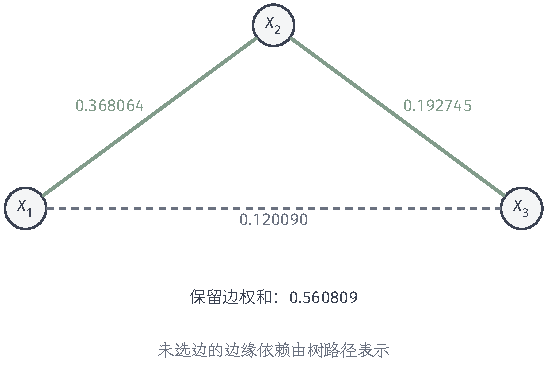
\includegraphics[width=92.650mm]{figures/06-probabilistic-graphical-models/03-learning/tikz/pgm-structure-learning-chow-liu/figure.pdf}
  \caption{计数表的互信息边权，单位为nat。最大权生成树保留实线两边，虚线是未选边。这个构造的经验分布恰好属于树族，因此可以精确复原；一般数据得到的是最佳树近似。}
  \label{fig:pgm-structure-learning-chow-liu}
\end{figure}

选$1$为根，根概率为$p(X_1=1)=0.5$，两条边的翻转概率为$0.1$、$0.2$。模型给出$\widehat p_{\mathcal{T}}(0,0,0)=0.5\times0.9\times0.8=0.36$；平均对数似然$-3\log2+0.368064+0.192745=-1.518633$，与前面评分计算相符。

证明中的正单点边缘用于保证条件概率分母有定义。零计数时可限制到经验支持，对从未出现的配置任选归一化条件表，并以$0\log0=0$延伸似然。若引入平滑伪计数，比较目标就随之改变。一般离散树的自由参数总数为
\[
  \sum_i(r_i-1)+
  \sum_{\{i,j\}\in E_{\mathcal{T}}}(r_i-1)(r_j-1).
\]
节点状态数相同等条件下，各树才有同一参数维数。状态数不同也不影响Chow--Liu对树族似然的精确优化，但BIC需扣除随边变化的参数惩罚，边权应作相应调整。

树约束同时简化学习与推断，也排除了环和不可约高阶作用。总体分布超出树族时，算法仍只能返回最佳树近似；互信息差异小时，抽样波动可能改变所选边。零权边也可能仅用于连接全节点，允许森林并惩罚边数则可保留断开的部分。

\subsection{高斯图结构学习}
\label{sec:pgm-structure-learning-gaussian}

连续变量的条件依赖在高斯情形也有简洁表示。取$\bm{X}\sim\mathcal{N}(\bm{\mu},\bm{\Sigma})$、$\bm{\Sigma}\succ0$，\term{精度矩阵}（precision matrix）$\bm{K}=\bm{\Sigma}^{-1}$的零元素满足
\[
  X_i\perp X_j\mid\bm{X}_{V\setminus\{i,j\}}
  \quad\Longleftrightarrow\quad K_{i,j}=0.
\]
协方差零表示高斯边缘独立，精度零表示给定其余变量后的独立，二者约束不同。离开高斯分布后，逆协方差一般也失去这项条件独立解释。

由样本计算$\widehat{\bm{\Sigma}}=n^{-1}\sum_r(\bm{x}_r-\overline{\bm{x}})(\bm{x}_r-\overline{\bm{x}})^{\top}$，高斯负对数似然去常数并缩放后成为$-\log\det\bm{K}+\operatorname{tr}(\widehat{\bm{\Sigma}}\bm{K})$。小样本协方差可能奇异，直接求逆通常也不给稀疏零模式。对各变量样本方差严格为正的情形，\term{图Lasso}（graphical lasso）取$\lambda>0$，用非对角稀疏惩罚估计正定精度矩阵：
\begin{equation}
  \widehat{\bm{K}}
  =\argmin_{\bm{K}\succ0}
    \left\{-\log\det\bm{K}
      +\operatorname{tr}(\widehat{\bm{\Sigma}}\bm{K})
      +\lambda\sum_{i\ne j}|K_{i,j}|\right\}.
  \label{eq:pgm-structure-learning-glasso}
\end{equation}
上述样本方差与正惩罚条件保证唯一的有限正定最优解。若取$\lambda=0$，则需$\widehat{\bm{\Sigma}}\succ0$，最优解为其逆矩阵；零样本方差的变量应先移除或另行建模。

惩罚跳过对角，同时计算两个对称非对角元；只对$i<j$求和的实现需要换算$\lambda$。正定约束保持合法密度，$\ell_1$项允许估计出现精确零。目标是凸函数，可以用凸优化方法求解，抽样误差及选边正确性仍需统计条件\scite{pgm-structure-learning-friedman2008}

还可从每个节点的条件预测选择邻居。高斯条件均值为
\[
  \mathbb{E}[X_i\mid\bm{X}_{-i}]
  =\mu_i+\sum_{j\ne i}
    \left(-\frac{K_{i,j}}{K_{i,i}}\right)(X_j-\mu_j),
\]
$-i$表示其余全部节点，回归系数的非零模式因而对应邻居。分别作稀疏回归后，两端可能对同一边作不同选择；OR取并集，较多保留边，AND取交集，较少保留边。联合密度还需对称正定的精度矩阵，因此各节点独立回归后应继续检查或拟合相容参数。

例如取以下精度与协方差：
\[
  \bm{K}=
  \begin{pmatrix}
    2&-1&0\\
    -1&2&-1\\
    0&-1&2
  \end{pmatrix},
  \qquad
  \bm{\Sigma}=\frac14
  \begin{pmatrix}
    3&2&1\\
    2&4&2\\
    1&2&3
  \end{pmatrix}.
\]
两矩阵相乘为单位阵，精度矩阵顺序主子式为$2,3,4$，故正定。$\Sigma_{1,3}=1/4$显示边缘相关，$K_{1,3}=0$则说明给定$X_2$后独立。节点$1$仅回归到$X_2$，系数$1/2$；节点$2$对两端的系数也均为$1/2$，得到同一链。实际调参应按用途评价$\lambda$，预测误差最小与精确选边可能需要不同取值。

\subsection{离散与高阶Markov网络结构学习}
\label{sec:pgm-structure-learning-discrete}

一般离散分布需要直接选择相互作用。先规定特征字典$\{f_a(\bm{x}_{C_a})\}$，$C_a\subseteq V$表示每个特征涉及的节点，再用有限状态的正指数模型表示概率：
\[
  p_{\bm{\theta}}(\bm{x})
  =\exp\!\left\{\sum_a\theta_a f_a(\bm{x}_{C_a})
                    -A(\bm{\theta})\right\}.
\]
参数的非零模式决定哪些相互作用参与模型。同一作用域有多项编码时，可用组稀疏惩罚共同选取；编码需可识别或有对比约束，使零系数具有确定含义。高阶因子的作用域在无向图中成为团，因此因子集合还能区分同一边图中的不同高阶关系。

用$\widehat{\mathbb{E}}[f_a]$表示经验特征均值，取$\lambda>0$并惩罚全部参数，完整似然的稀疏估计为
\[
  \min_{\bm{\theta}}\left\{
    A(\bm{\theta})-\sum_a\theta_a\widehat{\mathbb{E}}[f_a]
      +\lambda\lVert\bm{\theta}\rVert_1\right\}.
\]
正惩罚使参数趋于无穷时目标发散，从而存在有限最优参数。取$\lambda=0$时，需另查无罚最大似然估计是否存在；某些经验零频率会使目标仅在参数趋于无穷时逼近下确界。

梯度含模型期望，每轮都要进行推断；大团或大树宽会反复增加这项成本。\term{伪似然}（pseudolikelihood）改用各节点条件概率的乘积$\prod_{r,i}p_{\bm{\theta}}(x_{r,i}\mid\bm{x}_{r,-i})$。它只在单节点状态上归一化，可绕过全局配分函数；评价其统计效率与有限样本性质时，需要针对这个替代目标分析。

在成对Ising模型中，取$x_i\in\{-1,1\}$，局部场$u_i=b_i+\sum_{j\ne i}J_{i,j}x_j$汇总其他节点的作用。单点条件对数赔率为
\[
  \log\frac{p(X_i=1\mid\bm{x}_{-i})}
                {p(X_i=-1\mid\bm{x}_{-i})}=2u_i.
\]
该对数赔率使邻域估计化为稀疏逻辑回归。共同优化对称参数$J_{i,j}=J_{j,i}$时，条件概率来自同一联合模型；逐节点分别拟合时，还要协调两端选边与参数。直接搜索因子也可使用精确、近似或伪似然评分，应明确实际比较的目标。

成对边缘还可能隐藏高阶关系。以下正分布给出一个三变量反例：
\[
  p(x_1,x_2,x_3)
  =\frac{\exp(\theta x_1x_2x_3)}{8\cosh\theta},
  \qquad x_i\in\{-1,1\},\quad \theta\ne0.
\]
消去任一变量，分子变为$2\cosh\theta$，每对边缘都是$1/4$，故成对互信息为零。三阶矩却满足$\mathbb{E}[X_1X_2X_3]=\tanh\theta\ne0$，给定$X_3$后两端仍有相互作用。这个处处正的分布需要三阶特征，说明成对独立不足以推出联合独立。若允许大小至多$m$的作用域，候选子集数为$\sum_{\ell=1}^{m}\binom d\ell$，每个离散作用域还可能有多个参数，搜索及样本成本随之增长。

\subsection{潜变量结构}
\label{sec:pgm-structure-learning-latent}

稠密观测关系还可能由共同隐变量产生。将联合高斯节点分为观测集合$O$和潜变量集合$H$，按两组分块精度矩阵。积分潜变量或对二次型配方后，观测边缘的精度为
\begin{equation}
  \begin{aligned}
    \bm{K}_{\mathrm{marg}}
      &=(\bm{\Sigma}_{O,O})^{-1}\\
      &=\bm{K}_{O,O}
        -\bm{K}_{O,H}\bm{K}_{H,H}^{-1}\bm{K}_{H,O}\\
      &=\bm{S}-\bm{L}.
  \end{aligned}
  \label{eq:pgm-structure-learning-schur}
\end{equation}
$\bm{S}=\bm{K}_{O,O}$表示给定潜变量后的条件精度；$\bm{L}\succeq0$且秩至多$|H|$表示边缘化带来的修正。条件图稀疏、有效潜变量少时，这构成常称的\term{稀疏加低秩分解}（sparse plus low-rank decomposition）。名称强调两种结构，按此处半正定约定实际以减法组合。

取$X_i=Z+\varepsilon_i$，$i=1,2,3$，并令$Z,\varepsilon_1,\varepsilon_2,\varepsilon_3$相互独立且均为标准高斯。给定$Z$后三个观测独立；积分$Z$后协方差为$\bm{I}+\bm{1}\bm{1}^{\top}$，其逆可直接验证为
\[
  \bm{K}_{\mathrm{marg}}
  =\bm{I}-\frac14\bm{1}\bm{1}^{\top}.
\]
所有非对角元为$-1/4$，所以观测条件图完整，而$\bm{S}=\bm{I}$、$\bm{L}=\bm{1}\bm{1}^{\top}/4$只有一个潜在修正方向。边缘依赖与给定共同潜变量后的独立，描述的是不同条件分布。

根据观测样本协方差$\widehat{\bm{\Sigma}}_{O,O}$，取$\lambda>0$，可以同时拟合这两种结构：
\begin{equation}
  \begin{aligned}
    \min_{\bm{S},\bm{L}}\quad&
      -\log\det(\bm{S}-\bm{L})
      +\operatorname{tr}\!\left(
           \widehat{\bm{\Sigma}}_{O,O}(\bm{S}-\bm{L})\right)\\
      &+\lambda\bigl(\gamma\lVert\bm{S}\rVert_1
                      +\operatorname{tr}(\bm{L})\bigr),\\
    \text{满足}\quad&\bm{S}-\bm{L}\succ0,\qquad \bm{L}\succeq0.
  \end{aligned}
  \label{eq:pgm-structure-learning-sparse-low-rank}
\end{equation}
$\lVert\bm{S}\rVert_1$逐元素求绝对值，包含对角；$\gamma>0$调节稀疏与低秩惩罚的相对强度。正惩罚控制精度矩阵及潜变量修正的增长，使有限正定最优解存在。取$\lambda=0$时，仍需观测样本协方差正定，边缘精度的最优解才是其逆矩阵，$\bm S$与$\bm L$的分解则可能不唯一。

半正定矩阵的核范数等于迹，所以第二项鼓励低秩。该凸程序的恢复保证还需两类结构足够可区分，例如潜变量作用分散于较多观测节点，避免低秩项本身也高度稀疏\scite{pgm-structure-learning-chandrasekaran2012}

若某分量同时稀疏、低秩，它可以在两项间移动而不改变差，精确边缘精度也可能无法确定唯一分解。满足识别条件时，$\bm{L}$的秩表示有效潜在维数，潜变量的物理个数、旋转与含义仍需额外信息。完整潜变量图、条件图$\bm{S}$和边缘观测图$\bm{K}_{\mathrm{marg}}$因此应分别解释；低秩分解回答统计结构问题，尚未识别潜在因果机制。

\section{因果发现}
\label{sec:pgm-structure-learning-causal}

到这里，图用于表示联合分布。若要预测外部改变某变量的后果，还需给局部关系赋予干预含义。接下来比较不同信息与假设能识别到什么结构，让输出对应可以成立的因果结论。

\subsection{因果假设与识别目标}
\label{sec:pgm-structure-learning-causal-assumptions}

因果Markov性要求每个变量在给定其直接原因后，与非后代独立；忠实性则要求分布中的条件独立都由图上的d-分离解释。前者从机制导出独立约束，后者支持从独立关系反推图，但观测等价仍会限制方向识别（参见\BookSectionRef{sec:causal-generating-structure}{第一卷“数学准备”的生成结构推断节}）。本节在这些条件下考察可识别输出，再说明潜在混杂、函数形式及干预如何提供不同信息。

当前变量是否覆盖共同原因，也影响图的解释。\term{因果充分性}（causal sufficiency）要求它们的共同原因都已观测，即当前模型没有遗漏潜在混杂。它只针对所选节点集合，通常还需无环过程、已声明的数据环境及适当处理选择偏差。以函数形式识别更多方向时，还要加入相应线性、噪声独立或非高斯条件；搜索方法使用这些假设，却不能自行验证它们成立。

因果充分、无环且忠实时，观测独立信息一般确定CPDAG。允许潜变量后，需表示边缘化留下的关系。\term{最大祖先图}（maximal ancestral graph, MAG）用有向、双向及处理选择偏差时的无向边表达观测独立性，省去潜变量的显式细节。合法图无有向环；箭头端不能是另一端的祖先，无向边的端点不能再接指入箭头。“最大”表示每对不相邻节点都能由某组观测量分离。对应的\term{m-分离}（m-separation）按两侧箭头辨认路径碰撞点：活跃路径要求非碰撞点不在条件集中，每个碰撞点自身或某个后代在条件集中；两端没有活跃路径时才被分离。

多张MAG也可能具有相同独立关系，\term{部分祖先图}（partial ancestral graph, PAG）保留这类图共同的端点信息。尾端和箭头端为类内不变标记，圆圈表示端点尚未确定，边本身仍存在。无选择偏差时，$i\to j$表示祖先关系，$i\leftrightarrow j$排除互为祖先且与潜在混杂相容，$i\mathbin{\circ\!\!\to}j$只确定$j$端箭头。这些标记表达祖先与独立性的不确定性，未给出直接因果机制、双向反馈或潜变量的具体个数和连接\scite{pgm-structure-learning-zhang2008}

\subsection{基于观测数据的因果发现}
\label{sec:pgm-structure-learning-observational}

PC与GES得到的统计等价类，要在因果假设下才能解释为因果等价类（参见第~\ref{sec:pgm-structure-learning-directed}节）。PC在因果Markov性、忠实性、充分性、无环性及准确独立判定下返回CPDAG，有限样本返回其估计。GES则需要评分等价、可分解且局部一致，真实分布忠实于候选有向图，并满足固定维大样本条件。这里局部一致性具体指：样本足够多时，评分奖励补上遗漏依赖，惩罚多余依赖；在这些条件下等价类搜索可恢复CPDAG。

潜在混杂会改变需要检查的分离集合。\term{快速因果推断算法}（fast causal inference, FCI）扩展PC的搜索范围并采用祖先图定向规则，在相应Markov性、忠实性和准确独立信息下输出PAG。标准框架还可处理声明的选择机制。无限观测数据也可能只确定这个部分对象，圆圈应继续保留；完整规则及识别范围见Zhang的研究\scite{pgm-structure-learning-zhang2008-completeness}

分布形状可以提供独立关系之外的方向信息。\term{线性非高斯无环模型}（linear non-Gaussian acyclic model, LiNGAM）以独立扰动驱动各节点：
\[
  X_j=\sum_{i\in\operatorname{pa}(j)}b_{j,i}X_i+\varepsilon_j,
\]
图取无环，扰动相互独立、非高斯且方差有限非零，并排除未观测混杂。令$B_{j,i}=b_{j,i}$，递归方程给出$\bm{X}=(\bm{I}-\bm{B})^{-1}\bm{\varepsilon}$。\term{独立成分分析}（independent component analysis, ICA）利用源独立性分离混合观测；在这里非高斯性区分扰动，无环约束再处理相关排列歧义，于是可在模型条件下识别超出MEC的方向。线性高斯分布缺少这种方向信息，识别结论依赖所保留的非高斯条件\scite{pgm-structure-learning-shimizu2006}

非线性函数也可能使方向不对称。\term{加性噪声模型}（additive noise model, ANM）取$Y=f(X)+\varepsilon$、$\varepsilon\perp X$；在满足相应光滑性、非退化和可识别性条件的模型中，反向无法同时写成$X=g(Y)+\eta$、$\eta\perp Y$。因此可比较输入与拟合残差的独立性，而不只比较回归误差。多变量形式还需递归机制及独立扰动；线性高斯等双向可表示情形属于识别例外\scite{pgm-structure-learning-peters2014}

\subsection{基于干预数据的因果发现}
\label{sec:pgm-structure-learning-interventional}

观测和干预的差别可以继续用计数表说明。观测$X_2=1$时，$X_1=1$的频率为$0.9$；外部设置$X_2$却改变了数据产生方式。正向链$X_1\to X_2\to X_3$中，改变中间变量不影响其上游$X_1$；分叉$X_1\leftarrow X_2\to X_3$中，$X_1$随之改变。这类实验能区分相同被动观测支持的机制。

为计算这种改变，\term{完美干预}（perfect intervention）替换目标节点的机制、切断它对原父节点的依赖，同时保持其他机制。取已知目标集合$I\subseteq V$，各目标独立随机化并使用外部规定的$q_i^I$，干预分布为
\begin{equation}
  p^I(\bm{x})
  =\prod_{i\in I}q_i^I(x_i)
   \prod_{j\notin I}
      p(x_j\mid\bm{x}_{\operatorname{pa}_{\mathcal{G}}(j)}).
  \label{eq:pgm-structure-learning-intervention}
\end{equation}
图上删去进入$I$的全部箭头，得到$\mathcal{G}^{[I]}$；$I=\varnothing$给回观测环境。固定目标值可作为退化干预。以独立信息刻画等价类时，需要足够支持的随机化或覆盖相关取值的实验，以免变量固定造成额外退化。

记目标集合族为$\mathcal{I}$。若每个节点至少在一个环境未受干预，该族称为\term{保守的}（conservative），包含观测环境即满足。给定目标及完美干预规则后，允许相同多环境分布族的有向无环图构成\term{干预Markov等价类}（interventional Markov equivalence class, I-MEC）。各环境共享非目标机制，因而这里比较的是协调的多环境模型。

在保守目标族及相应正性条件下，两图干预等价恰好要求观测Markov等价，并且每个$I\in\mathcal{I}$下的删入边图具有相同骨架。也可用观测骨架与v-结构相同，再比较各干预图的Markov等价关系来刻画。\term{干预本质图}（interventional essential graph）把I-MEC共同方向画成箭头，其余边保持无向。干预细分了观测MEC，但目标不足时仍可能保留多张候选图\scite{pgm-structure-learning-hauser2012}

将三种观测等价图都拟合到同一二值表，再作$\operatorname{do}(X_2=1)$。正向链预测$(p(X_1=1),p(X_3=1))=(0.5,0.8)$，分叉为$(0.9,0.8)$，反向链为$(0.9,0.5)$；仅观测$X_2=1$时，三者却都给$(0.9,0.8)$。图~\ref{fig:pgm-structure-learning-intervention}展示这组差异：在给定总体假设下，覆盖$X_2$两种取值的完美干预足以区分它们。有限实验还需评价频率估计误差。

\begin{figure}[htbp]
  \centering
  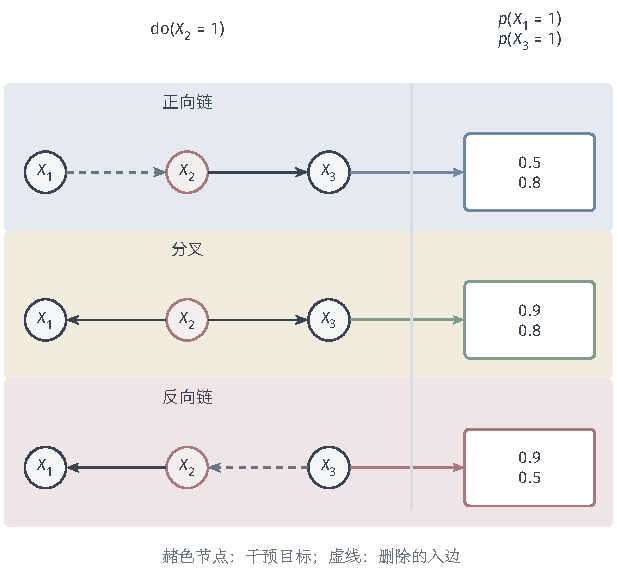
\includegraphics[width=104.405mm]{figures/06-probabilistic-graphical-models/03-learning/tikz/pgm-structure-learning-intervention/figure.pdf}
  \caption{干预$X_2$对同一观测MEC的三种预测。蓝、黄、红横带依次为正向链、分叉、反向链，右侧概率框以同色箭头与结构对应。实线保留非目标机制，虚线表示切断的入边；在给定三节点设定下，预测差异提供方向信息。}
  \label{fig:pgm-structure-learning-intervention}
\end{figure}

\term{贪心干预等价搜索}（greedy interventional equivalence search, GIES）直接在干预本质图空间比较I-MEC，采用前向、后向及转向操作。每条记录需带目标标签$I_r$；目标随机化分布已知或独立于候选图时，去掉共同常数后的机制对数似然为
\[
  \ell(\mathcal{G},\bm{\theta})
  =\sum_{r=1}^{n}\sum_{j\notin I_r}
       \log p_{\bm{\theta}_j}
          (x_{r,j}\mid\bm{x}_{r,\operatorname{pa}(j)}).
\]
目标节点的观测不用于拟合它的原机制，仍可进入子节点的机制拟合。各机制可用样本数不同，惩罚评分需要体现这种多环境设定。GIES据此汇合观测与干预证据；具体搜索最优性及因果恢复仍须结合评分、样本和模型条件分析。

未知目标时，环境标签只说明有机制变化，还需限定哪些机制可变、变化是否可检测及其余机制如何保持，再联合推断目标。软干预只改机制的一部分而保留父依赖，也需要修改删边表示和I-MEC定义。执行不依从、目标不完全、非目标机制漂移或潜在混杂都会改变识别范围，应使用与这些条件相容的模型。

已有候选还可用于决定下一次实验。\term{主动实验设计}（active experimental design）在可执行且满足预算的目标中，选择预计最能区分候选的干预；三节点例子的中间节点就是一项选择。预期后验熵下降、待定端点减少或科学查询的区分度都可作为准则，并需计入成本。这些预期仍依赖当前模型和机制不变假设，实验实施后的证据要另外评价。

表~\ref{tab:pgm-structure-learning-causal-routes}把信息、假设和输出放在同一口径下比较。路线可以交叉：ANM可使用回归及独立检验，连续优化也可处理特定函数模型。识别能力由数据和模型条件决定，求解工具规定如何利用这些信息。

\begin{table*}[htbp]
  \centering
  \small
  \begin{tabularx}{\linewidth}{@{}lXX@{}}
    \toprule
    路线 & 关键条件与信息 & 理想识别对象及限制 \\
    \midrule
    PC & 无环、因果充分、Markov且忠实；准确独立性信息 & CPDAG；不决定类内可逆方向 \\
    GES & 相应充分有向图模型；评分等价、可分解、局部一致 & 大样本下CPDAG；不是一般贪心搜索的保证 \\
    FCI & 允许潜在混杂；相应Markov性、忠实性及选择机制假设 & PAG；不是潜变量完整图 \\
    LiNGAM & 线性无环、独立非高斯扰动、无潜在混杂 & 模型条件下单个有向图；依赖分布形状 \\
    ANM & 独立加性噪声、无混杂及特定可识别性条件 & 满足条件时单个有向图；存在双向可表示例外 \\
    GIES & 已知目标的完美干预、无混杂、机制不变、相应评分 & 搜索I-MEC；并非一般全局最优保证 \\
    \bottomrule
  \end{tabularx}
  \caption{不同假设下的识别目标。表列理想输出以总体条件成立为前提；实际估计还包含抽样、拟合与搜索误差，因此需同时说明假设和计算过程。}
  \label{tab:pgm-structure-learning-causal-routes}
\end{table*}

\subsection{因果发现的边界}
\label{sec:pgm-structure-learning-causal-limits}

不确定性需要按来源判断。样本误差使检验和评分偏离总体结果，增加同类记录有机会降低它。假设错误可能让更多数据稳定地支持错误图，例如有混杂却使用充分性模型。总体不可识别则意味着多个候选在所有允许资料下都产生同一分布，需要增加信息才能区分。这三种情况分别指向补样本、改模型及设计实验。

等价类中的未定向边和PAG圆圈保留的是资料尚未确定的信息。领域知识可以排除候选，应标明它贡献的方向；函数形式可以缩小等价范围，也需核验对应假设。稀疏、有向且重复得到的图仍只说明特定流程的结果，因果解释需要这些额外依据。

结构发现之后，干预效应是否可计算仍是另一项识别问题，do演算和反事实查询有各自定义及条件。本节得到的部分结构为这些查询提供约束，具体效应和个体反事实还需按对应问题分析。

\section{算法分析}
\label{sec:pgm-structure-learning-analysis}

评价结构学习可以沿三个问题展开：候选图及局部函数能表示哪些分布；搜索能否找到目标候选、以多少计算完成；有限样本下选出的结构与预测能否接近总体目标。下面分别检查统计一致性、计算成本和评价协议，使“最优”“一致”与“稳定”各有明确对象。

\subsection{统计一致性与有限样本误差}
\label{sec:pgm-structure-learning-consistency}

先把可识别目标记为$\mathcal{C}^{*}$，例如CPDAG；\term{结构一致性}（structural consistency）要求$\mathbb{P}(\widehat{\mathcal{C}}_n=\mathcal{C}^{*})\to1$。目标必须与可用信息匹配。真实分布超出树族时，Chow--Liu可以趋向最佳树近似；图Lasso参数误差趋零时，精确零模式还需非零信号与零之间有足够间隔。

PC需要全部相关独立判定同时正确。若检验集合大小为$M$、每项错误概率至多$\delta$，联合界给出至少一项检验出错的概率至多$M\delta$，无需检验独立。自适应选择时应覆盖全部可能用到的检验，而非事后只数执行次数。若要整体错误随$n$消失，固定显著性水平通常不足，还需合适阈值序列及功效条件。

最弱依赖往往决定可恢复程度。高斯偏相关小于估计波动时难以检出；离散条件集扩大后，每个配置的记录更少。稀疏图有助于限制条件集，同时仍需控制最大度、状态数、协方差条件数或最小信号，才能给出具体一致性结论。

BIC比较也依赖固定维、正确模型和正则条件。遗漏依赖通常带来随$n$线性增长的似然损失，多余参数的随机拟合收益通常仅为有界概率量级，$\log n$惩罚据此区分两者。这个理由说明评分的候选比较；搜索若未到达相关模型，还需另外控制搜索误差。潜变量奇异或维数增长时，应重查渐近尺度。

树的稳定性可以由边权间隔直接说明。取$d\geq3$且总体最大权生成树唯一，对非树边$e$与其连接路径上的树边$f$，定义
\[
  \Delta=\min_{e\notin E_{\mathcal{T}^{*}}}
             \min_{f\in\operatorname{path}_{\mathcal{T}^{*}}(e)}
             \{I_f-I_e\}.
\]
若$\Delta>0$且所有互信息估计误差小于$\Delta/2$，非树边与路径边的次序保持，最大权树也保持。教学例子中间隔约为$0.072654$，等于较小两条互信息的差。零间隔可能容许多棵最优树，分布预测相近时具体选边仍可能变化。

\subsection{计算复杂度与可扩展性}
\label{sec:pgm-structure-learning-complexity}

计算成本要按实际搜索规模估计。PC枚举条件集并逐项检验；整个过程中候选邻域至多$q$时，粗略检验数为$O(d^2 2^q)$，总时间还乘单次检验成本。误保留边会增大候选邻域，故$q$未必等于真实最大度。FCI扩大了分离集搜索范围，也增加相应运算。

离散有向图可缓存局部评分，候选父集数量仍可能指数增长。预计算最佳父集表后，常见动态规划递推约需$O(d2^d)$时间，表的准备及内存另计；整数规划的分支搜索同样可能指数增长。局部搜索每轮约检查$O(d^2)$个移动，总成本还取决于轮数、无环检查及拟合，需与单轮操作数分开。

状态数有界时，Chow--Liu以$O(nd^2)$时间汇总成对计数，再以稠密Prim的$O(d^2)$或排序Kruskal的$O(d^2\log d)$求树。固定树上的有限状态边缘推断随节点数线性增长。这两项计算收益来自树约束，也伴随其表示能力限制。

稠密NOTEARS每次残差乘法约需$O(nd^2)$，矩阵指数通常需$O(d^3)$规模的线性代数，总时间还乘内部优化及惩罚更新轮数。图Lasso有矩阵更新成本，凸性则方便检查求解误差；逐节点回归易并行，联合参数相容性需继续处理。高阶离散评分还可能反复计算配分函数。限制父集或作用域时，应说明节省的计算和排除的候选。

\subsection{结构评价与稳定性}
\label{sec:pgm-structure-learning-evaluation}

仿真有已知生成结构时，可分别测量骨架与方向。骨架精确率为正确边数除以预测边数，召回率为正确边数除以真实边数，零分母规则需预设。方向评价需说明是否计入漏边。若资料只能识别CPDAG，应以该类为目标，既不因未选中某代表的可逆方向罚分，也不把偶然猜中当作识别收益。

\term{结构Hamming距离}（structural Hamming distance, SHD）计量估计图变到目标图所需的边编辑数。常见约定将加边、删边、反向各计1，也有把反向计为删加两步的实现，比较时需固定口径。CPDAG评价先将生成有向图转为等价类，再比较邻接、被迫方向和未定向状态；PAG还需比较圆圈、尾端及箭头端。

真实记录缺少标准答案时，可测量结果对重采样的敏感性。\term{自助重采样}（bootstrap）从$n$条独立记录有放回抽$n$条，重复拟合$B$次，将边出现频率写为
\[
  \widehat\pi_{i,j}
  =\frac1B\sum_{b=1}^{B}
       \mathbf{1}\{\{i,j\}\text{在第}b\text{次结果中相邻}\}.
\]
方向需另计频率，并声明分母取全部重复还是该边出现的重复。CPDAG未定向边应保留该状态；各轮是否重做筛选与调参，也影响所测流程。多环境资料在环境内重采样，相关序列则按适当块抽样，使评价单位符合数据依赖。

重采样频率表示流程对数据扰动的敏感性；错误先验或模型假设也可能产生稳定结果，因此它不同于结构后验及因果真实性概率。还可比较合理正则、检验和模型设置，并在未参与选图与调参的记录上报告平均预测对数概率或对数密度，值越大表示给真实观测的预测支持越高。这项预测评价仍未验证因果方向。

领域知识也可明确限制候选。禁止$i\to j$就排除$X_j$父集中含$X_i$的选项，必选$i\to j$则保留包含$X_i$的父集；时间顺序排除逆时间箭头。搜索前需检查约束相容且无环；等价类结果还应区分数据确定与知识补充的方向，并相对于加入同一知识后的识别目标评价。

\section{本章小结}
\label{sec:pgm-structure-learning-summary}

从记录到图，需要分别判断局部独立证据、整体模型得分和合法空间搜索。检验说明哪些联系可由给定变量隔断，评分权衡拟合与复杂度，搜索组织候选比较。树之所以可精确求解，是因为最优似然化为互信息边权和；一般有向图和高阶无向模型还要承担更大的搜索或归一化成本。

同一张计数表可支持无向链、观测等价类及结构后验，却不能仅由频率选定因果方向。缺失观测引入后验统计量，潜变量边缘化可能使稀疏条件图变稠密；改变的不只是运算，也包括可识别对象。赋予结构因果解释时，需明确机制、混杂、忠实性和函数形式假设，才能判断结果是CPDAG、PAG还是干预等价类中的信息。

回到设备记录，数据能够帮助选择依赖表示，故障传播方向还需相应识别条件和干预依据。增加同类样本可以在相应统计条件下降低估计误差；改善搜索用于控制优化误差，修改假设用于处理模型偏差，总体观测等价则可能仍需新实验。因此报告结构时，应同时给候选范围、数据与干预条件、检验或评分、搜索限制及保留的不确定性。

接下来的模型以具体任务选择这些结构：分类、潜在分组和状态估计各需要怎样的表达与计算？静态有向模型把局部分解、推断和学习用于此类任务（参见第~\ref{chap:pgm-static-directed}章）。结构适合计算和预测时，潜变量的物理含义仍可能需要其他证据。

\paragraph{扩展阅读}
Koller与Friedman的教材进一步展开条件独立检验与评分搜索，可按本章的计数、等价类和搜索目标继续阅读。理解统计分解之后，再核对因果解释增加了哪些机制与识别条件\scite{pgm-koller2009}
